\documentclass[a4paper, 12pt]{article}
\usepackage{eurosym}
\usepackage{pdflscape}
\usepackage{pgfgantt}
\usepackage{pgfplots}


\newcommand{\templates}{../../template}
\usepackage[a4paper, margin=2.5cm]{geometry}

\usepackage{enumitem}
\setlist[itemize]{noitemsep}
\setlist[enumerate]{noitemsep}

\let\oldpar\paragraph
\renewcommand{\paragraph}[1]{\oldpar{#1\\}\noindent}

% Avoid dots in the table of contents, it mess with the gulpease calculation
\makeatletter
\renewcommand{\@dotsep}{10000} 
\makeatother
\usepackage{graphicx}
\usepackage{hyperref}
\usepackage{makecell}
\usepackage{fancyhdr}

\newcommand{\settitolo}[1]{\newcommand{\titolo}{#1\\}}
\newcommand{\setprogetto}[1]{\newcommand{\progetto}{#1\\}}
\newcommand{\setcommittenti}[1]{\newcommand{\committenti}{#1\\}}
\newcommand{\setredattori}[1]{\newcommand{\redattori}{#1\\}}
\newcommand{\setrevisori}[1]{\newcommand{\revisori}{#1\\}}
\newcommand{\setresponsabili}[1]{\newcommand{\responsabili}{#1\\}}
\newcommand{\setversione}[1]{
	\ifdefined\versione\renewcommand{\versione}{#1\\}
	\else\newcommand{\versione}{#1\\}\fi
}
\newcommand{\setdestuso}[1]{\newcommand{\uso}{#1\\}}
\newcommand{\setdescrizione}[1]{\newcommand{\descrizione}{#1\\}}

\newcommand{\makefrontpage}{
	\begin{titlepage}
		\begin{center}

		
\includegraphics[width=0.4\textwidth]{\templates/4ourSquared_logo}\\

		{\Large 4OURSQUARED}\\[6pt]
		\href{mailto://4oursquared.unipd@gmail.com}{4oursquared.unipd@gmail.com}\\
		
		\ifdefined\progetto
		\vspace{1cm}
		{\Large\progetto}
		{\large\committenti}
		\else\fi
		
		\vspace{1.5cm}
		{\LARGE\titolo}
		
		\vfill
		
		\begin{tabular}{r | l}
		\multicolumn{2}{c}{\textit{Informazioni}}\\
		\hline
		
		\ifdefined\redattori
			\textit{Redattori} &
			\makecell[l]{\redattori}\\
		\else\fi
		\ifdefined\revisori
			\textit{Revisori} &
			\makecell[l]{\revisori}\\
		\else\fi
		\ifdefined\responsabili
			\textit{Responsabili} &
			\makecell[l]{\responsabili}\\
		\else\fi
		
		\ifdefined\versione
			\textit{Versione} & \versione
		\else\fi
		
		\textit{Uso} & \uso
		
		\end{tabular}
		
		\vspace{2cm}
		
		\ifdefined\descrizione
		Descrizione
		\vspace{6pt}
		\hrule
		\descrizione
		\else\fi
		\end{center}
	\end{titlepage}
}
\usepackage{hyperref}
\usepackage{array}
\usepackage{tabularx}
\usepackage{adjustbox}

\newcounter{verscount}
\setcounter{verscount}{0}
\newcommand{\addversione}[5]{
	\ifdefined\setversione
		\setversione{#1}
	\else\fi
	\stepcounter{verscount}
	\expandafter\newcommand%
		\csname ver\theverscount \endcsname{#1&#2&#3&#4&#5}
}

\newcommand{\listversioni}{
	\ifnum\value{verscount}>1
		\csname ver\theverscount \endcsname
		\addtocounter{verscount}{-1}
		\\\hline
		\listversioni
	\else
		\csname ver\theverscount \endcsname\\\hline
	\fi
}

\newcommand{\makeversioni}{
	\begin{center}
		\begin{tabularx}{\textwidth}{|c|c|c|c|X|}
		\hline
		\textbf{Versione} & \textbf{Data} & \textbf{Redattore} & \textbf{Verificatore} & \textbf{Descrizione} \\
		\hline
		\listversioni
		\end{tabularx}
	\end{center}
	\clearpage
}
\graphicspath{ {./immagini/} }

\settitolo{Piano di Progetto}
\setredattori{Alberti Nicolas \\ Brotto Romina \\ Cavaliere Erica \\ Soldà Matteo}
\setdestuso{esterno}
\setdescrizione{
Questo documento serve a tracciare l'efficienza del progetto. Tiene traccia dei costi sostenuti fino ad oggi e li confronta con i costi preventivati, in relazione agli obiettivi fissati.
}

\addversione{0.0.1}{22/04/2023}{Cavaliere Erica}{Alberti Nicolas}{Stesura iniziale}
\addversione{0.0.2}{24/04/2023}{Cavaliere Erica}{Soldà Matteo}{Correzione errori e aggiunta delle intestazioni e dei piè di pagina}
\addversione{0.0.3}{26/04/2023}{Cavaliere Erica}{Brotto Romina}{Inserimento interruzioni di pagina e completamento grafico di Gantt}
\addversione{0.0.4}{16/05/2023}{Cavaliere Erica}{Salami Lorenzo}{Inserimento degli sprint e aggiornamento dei grafici di Gantt}
\addversione{0.0.5}{25/05/2023}{Alberti Nicolas}{Cavaliere Erica}{Inserimento dello sprint 4; aggiornamento dei grafici di Gantt}
\addversione{0.0.6}{02/06/2023}{Brotto Romina}{Soldà Matteo}{Completamento sprint 5}
\addversione{0.0.7}{11/06/2023}{Cavaliere Erica}{Soldà Matteo}{Completamento sprint 6}
\addversione{0.0.8}{23/06/2023}{Alberti Nicolas}{Cavaliere Erica}{Completamento sprint 7}
\addversione{0.0.9}{21/07/2023}{Soldà Matteo}{Cavaliere Erica}{Completamento sprint 8}
\addversione{0.0.10}{21/07/2023}{Soldà Matteo}{Alberti Nicolas}{Aggiunta di specifiche relative ai rischi}
\addversione{0.1.0}{24/07/2023}{Brotto Romina}{Soldà Matteo}{Verifica documento per RTB}
\addversione{1.0.0}{27/07/2023}{Soldà Matteo}{Brotto Romina}{Approvazione documento per RTB}
\addversione{1.0.1}{27/07/2023}{Brotto Romina}{Alberti Nicolas }{Aggiunta sprint e sezioni 2.2 e 2.3}
\addversione{1.0.2}{20/09/2023}{Salami Lorenzo}{Cavaliere Erica }{Completato piano di progetto}

\def\pgfcalendarmonthitname#1{%
\ifcase#1 \or Gennaio\or Febbraio\or Marzo\or Aprile\or Maggio\or Giugno\or Luglio\or Agosto\or Settembre\or Ottobre\or Novembre\or Dicembre\fi%
}
\usepgfplotslibrary{dateplot}

\begin{document}
\makeindexdetails
\makefrontpage \makeversioni
\tableofcontents
\newpage

\makecontentsdetails{Piano di Progetto}

\section{Analisi dei rischi}

\subsection{Rischi tecnologici}
Le tecnologie consigliate per lo svolgimento del progetto da parte del richiedente possono risultare nuove per alcuni componenti del gruppo, questo può portare difficoltà nell'utilizzo delle tecnologie, portando di conseguenza errori nel codice e ritardi di consegna. \newline
Per prefissare le scadenze bisognerà tenere conto del tempo impiegato per imparare le nuove tecnologie, oltre al tempo di sviluppo del progetto stesso.

\begin{center}
	\begin{tabularx}{\textwidth}{||c|X|X|c|c||}
		\hline
		\textbf{ID} & \textbf{Tipo}                          & \textbf{Descrizione}                                                                                                                                                                                                                  & \textbf{Frequenza} & \textbf{Gravità} \\
		\hline \hline
		RT1         & Inesperienza con linguaggi e framework & Questo rischio nasce dalla poca esperienza avuta sia con i linguaggi utilizzati e dalla esperienza nulla con i framework per l'intero team.                                                                                           & Alta               & Medio            \\
		\hline
		RT2         & Incompatibilità software               & Questo rischio nasce dalla differenza sia hardware che software tra i computer dei vari membri del team. Come accaduto in fase di sviluppo del \textit{PoC}, alcune versioni del database non sono compatibili con processori datati. & Bassa              & Alto             \\
		\hline \hline
	\end{tabularx}
\end{center}

\subsection{Rischi organizzativi}
Durante lo svolgimento del progetto, è possibile andare incontro a dei problemi di organizzazione degli orari e quindi di non riuscire a rispettare la stima delle ore richiesta e, di conseguenza, sforare i costi indicati dal preventivo iniziale.

\begin{center}
	\begin{tabularx}{\textwidth}{||c|X|X|c|c||}
		\hline
		\textbf{ID} & \textbf{Tipo}           & \textbf{Descrizione}                                                                                               & \textbf{Frequenza} & \textbf{Gravità} \\
		\hline \hline
		RO1         & Suddivisione del lavoro & Distribuzione non equa del lavoro dovuta all'inesperienza.                                                         & Media              & Medio            \\
		\hline
		RO2         & Impegni personali       & Problemi personali legati ad un singolo membro del gruppo o che possono includere più membri del team (es: esami). & Alta               & Medio            \\
		\hline
		RO3         & Conflitti interni       & Differenze nella soluzione proposta dai membri del team per la risoluzione di un problema                          & Bassa              & Medio            \\
		\hline \hline
	\end{tabularx}
\end{center}



\subsection{Rischi derivanti dai Requisiti}
Questi sono dovuti continuo mutamento dei requisti dovuti alla ricerca della soluzione che meglio si adatti alle richieste del committente e alla possibile malcomprensione dei requisiti stessi

\begin{center}
	\begin{tabularx}{\textwidth}{||c|X|X|c|c||}
		\hline
		\textbf{ID} & \textbf{Tipo}                  & \textbf{Descrizione}                                                                                     & \textbf{Frequenza} & \textbf{Gravità} \\
		\hline \hline
		RR1         & Incomprensione del requisito   & Comprensione errata del requisito richiesto dal proponente.                                              & Media              & Medio            \\
		\hline
		RR2         & Incompletezza del requisito    & Il capitolato potrebbe riportare in maniera ambigua o con mancanza di precisione il requisito richiesto. & Bassa              & Alto             \\
		\hline
		RR3         & Indisponibilità del proponente & Mancanza di tempo per il proponente per il supporto e la risoluzione di incomprensioni.                  & Bassa              & Medio            \\
		\hline \hline
	\end{tabularx}
\end{center}

\subsection{Prevenzione dei Rischi e Risoluzione dei Problemi}
\begin{center}
	\begin{tabularx}{\textwidth}{||c|c||X||}
		\hline
		\textbf{ID} & \textbf{Gravità} & \textbf{Prevenzione / Risoluzione}                                                                                                                                                                                      \\
		\hline \hline
		RT1         & Media            & Il team di sviluppo si impegna a familiarizzare autonomamente con i linguaggi e con i framework prescelti prima di apportare modifiche al codice sorgente del progetto                                                  \\
		\hline
		RT2         & Alta             & Qualora sorgesse una incompatibilità, in base al numero di membri del gruppo coinvolti, si valuterà attentamente tramite una riunione quale sia la soluzione più efficace per la risoluzione                            \\
		\hline
		RO1         & Media            & Qualora venisse segnalata questo tipo di inequità, il Responsabile provvederà alla riorganizzazione del lavoro                                                                                                          \\
		\hline
		RO2         & Media            & Il Responsabile provvede a riorganizzare il lavoro secondo disponibilità                                                                                                                                                \\
		\hline
		RO3         & Media            & Attraverso una riunione, il gruppo discute le soluzioni proposte e dopo una valutazione critica delle soluzioni, si procede ad una votazione con la quale selezionare l'approccio favorito dalla maggior parte del team \\
		\hline
		RR1         & Media            & Il gruppo nella sua interezza valuta il requisito per cercare una interpretazione unanime. Qualora il precedente approccio si rivelasse inconcludente, si procederà alla richiesta di un incontro con il proponente     \\
		\hline
		RR2         & Alta             & Il gruppo nella sua interezza si dedica alla valutazione del requisito. Qualora il precedente approccio si rivelasse inconcludente, si procederà alla richiesta di un incontro con il proponente                        \\
		\hline
		RR3         & Media            & Attraverso una riunione con il proponente, si cercherà di trovare un punto di accordo per quanto riguarda sia le modalità di comunicazione che le tempistiche                                                           \\
		\hline \hline
	\end{tabularx}
\end{center}

\newpage
\section{Pianificazione del lavoro}

\subsection{Lavoro svolto}
%Di seguito sono riportati i grafici aggiornati del lavoro pianificato.\newline
%Se si desidera vedere l'evoluzione degli impegni presi in un arco temporale preciso, lo si può vedere nella sezione \ref{Scrum}.\newline



\begin{itemize}
	\item Way of Working\newline
	      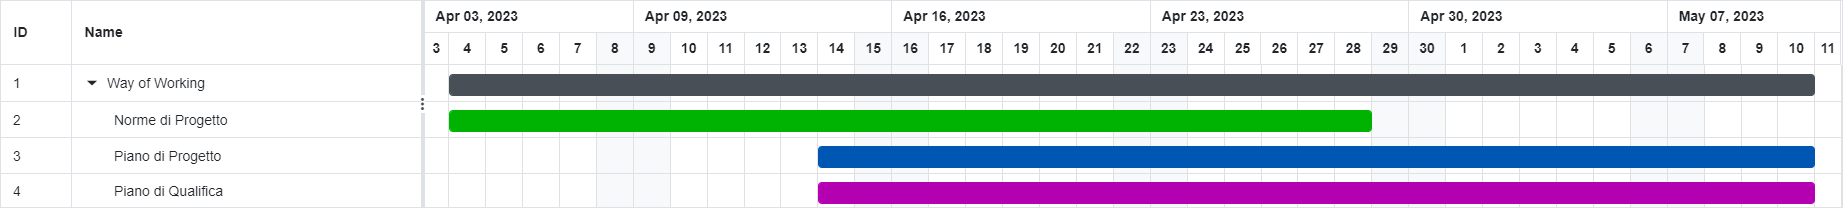
\includegraphics[scale=0.24]{WoW_2.png}\newline
	\item Requirements and Technology Baseline\newline
	      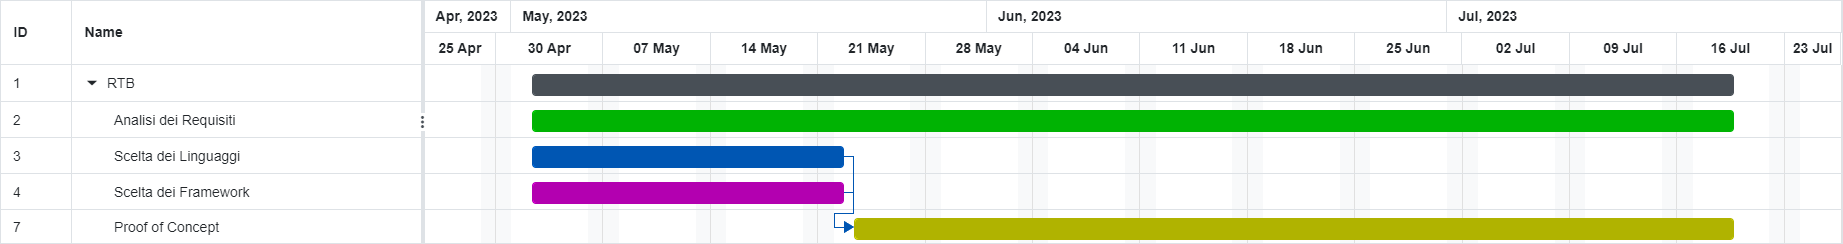
\includegraphics[scale=0.24]{RTB_9.png}\newline
\end{itemize}

\subsection{Stato di avanzamento corrente}
Attualmente il gruppo sta procedendo con l'implementazione delle funzionalità mancanti della Web Application. In particolare si stanno consolidando le funzionaloità di modifica della luminosità temportizzata e la gestione di login e logout.
La documentazione viene aggiornata in base al progresso dello stato di avanzamento.

\subsection{Metodo di lavoro}
Il framework Scrum è la modalità scelta dal gruppo per la gestione del lavoro.
Per ogni sprint saranno visibili:
\begin{itemize}
	\item Data di inizio e fine sprint
	\item Suddivisione del lavoro
	\item Difficoltà incontrate
	\item Diagramma di Gantt
	\item Tabelle di preventivo ore/costi e per membro
\end{itemize}

N.B.: il gruppo ha preso atto che alcuni sprint potranno essere meno produttivi di altri, a causa delle difficoltà che verranno incontrate nel percorso di sviluppo.


\newpage

\subsection{Scrum}\label{Scrum}

\subsubsection{Sprint 1}
\textbf{Data di inizio:} 14/04/2023\newline
\textbf{Data di fine:} 27/04/2023\newline
\newline
\textbf{Suddivisione del lavoro:}
\begin{itemize}
	\item aggiornamento delle norme di progetto;
	\item stesura del piano di progetto;
	\item stesura del piano di qualifica.
\end{itemize}
\textbf{Difficoltà incontrate:}
\begin{itemize}
	\item problemi a suddividere i ruoli e assegnare i compiti.
\end{itemize}
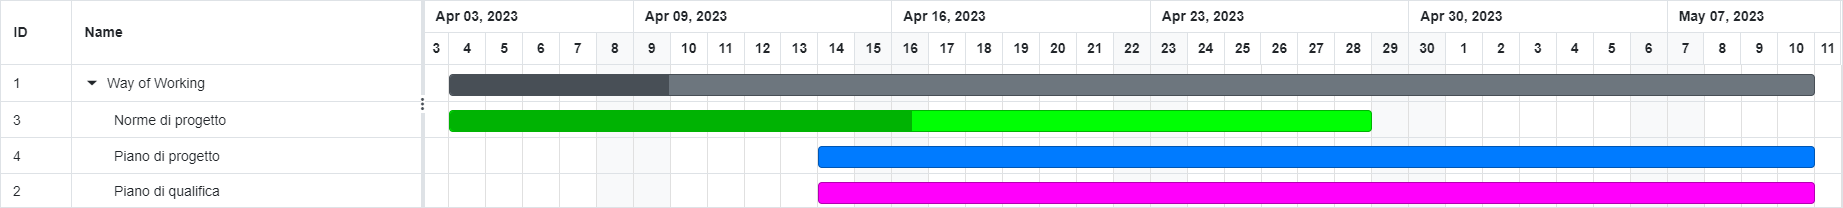
\includegraphics[scale=0.24]{WoW_1.png}\newline
\newline

\begin{center}
	\begin{tabularx}{\textwidth}{|X|X|X|X|}
		\hline
		\multicolumn{4}{|c|}{\textbf{Preventivo ore/costi}}                                      \\
		\hline
		\hline
		\textbf{Ruolo}  & \textbf{Costo orario (\euro)} & \textbf{Ore} & \textbf{Prezzo (\euro)} \\
		\hline
		Responsabile    & 30                            & 6(+6)        & 180                     \\
		\hline
		Amministratore  & 20                            & 4(+4)        & 80                      \\
		\hline
		Analista        & 25                            & 11(+11)      & 275                     \\
		\hline
		Progettista     & 25                            & 0(+0)        & 0                       \\
		\hline
		Programmatore   & 15                            & 0(+0)        & 0                       \\
		\hline
		Verificatore    & 15                            & 3(+3)        & 45                      \\
		\hline
		\hline
		\textbf{Totale} &                               & 24           & 580                     \\
		\hline
	\end{tabularx}\\[8pt]
	\mbox{}\\
\end{center}

\begin{center}
	\begin{tabularx}{\textwidth}{|X|X|X|X|X|X|X|}
		\hline
		\multicolumn{7}{|c|}{\textbf{Preventivo ore per membro}}                                \\
		\hline
		\hline
		\textbf{Membro}   & \textbf{Resp.}    & \textbf{Amm.}   & \textbf{Ana.} &
		\textbf{Proget.}  & \textbf{Program.} & \textbf{Verif.}                                 \\
		\hline
		Alberti Nicolas   & 0                 & 2(+2)           & 0             & 0 & 0 & 0     \\
		\hline
		Brotto Romina     & 0                 & 0               & 0             & 0 & 0 & 3(+3) \\
		\hline
		Cavaliere Erica   & 0                 & 0               & 5(+5)         & 0 & 0 & 0     \\
		\hline
		Ceccato Francesco & 0                 & 2(+2)           & 0             & 0 & 0 & 0     \\
		\hline
		Salami Lorenzo    & 0                 & 0               & 6(+6)         & 0 & 0 & 0     \\
		\hline
		Soldà Matteo      & 6(+6)             & 0               & 0             & 0 & 0 & 0     \\
		\hline
		\hline
		\textbf{Totale}   & 6(+6)             & 4(+4)           & 11(+11)       & 0 & 0 & 3(+3) \\
		\hline
	\end{tabularx}\\[8pt]
	\mbox{}\\
\end{center}

\newpage

\subsubsection{Sprint 2}
\textbf{Data di inizio:} 28/04/2023\newline
\textbf{Data di fine:} 08/05/2023\newline
\newline
\textbf{Suddivisione del lavoro:}
\begin{itemize}
	\item aggiornamento delle Norme di Progetto inserendo la gestione dei processi e il ticketing;
	\item creare una prima stesura dell'Analisi dei Requisiti;
	\item preparare una base delle Use Case da inserire nell'Analisi dei Requisiti;
	\item stesura di un Glossario.
\end{itemize}
\textbf{Difficoltà incontrate:}
\begin{itemize}
	\item iniziale difficoltà di organizzazione del lavoro;
	\item difficoltà nell'interpretazione di alcuni termini  del capitolato.
\end{itemize}
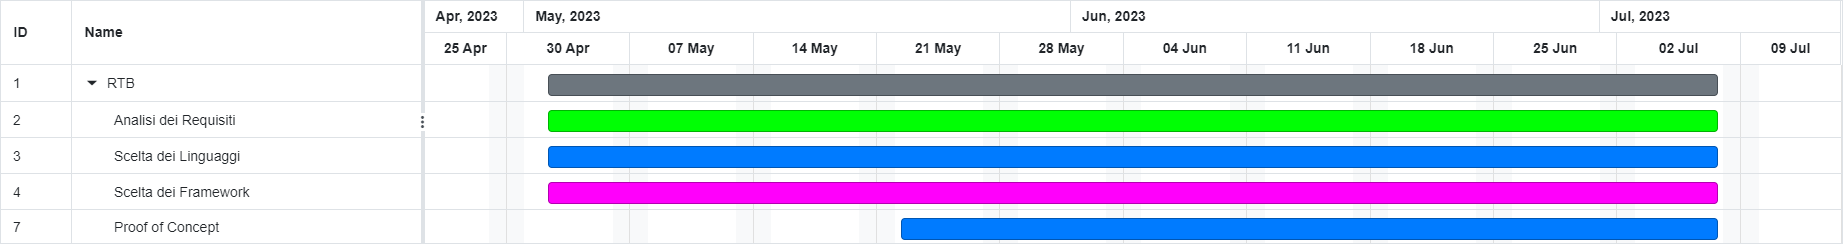
\includegraphics[scale=0.24]{RTB_1.png}\newline
\newline

\begin{center}
	\begin{tabularx}{\textwidth}{|X|X|X|X|}
		\hline
		\multicolumn{4}{|c|}{\textbf{Preventivo ore/costi}}                                      \\
		\hline
		\hline
		\textbf{Ruolo}  & \textbf{Costo orario (\euro)} & \textbf{Ore} & \textbf{Prezzo (\euro)} \\
		\hline
		Responsabile    & 30                            & 12(+6)       & 180                     \\
		\hline
		Amministratore  & 20                            & 9(+5)        & 100                     \\
		\hline
		Analista        & 25                            & 21(+10)      & 250                     \\
		\hline
		Progettista     & 25                            & 0(+0)        & 0                       \\
		\hline
		Programmatore   & 15                            & 0(+0)        & 0                       \\
		\hline
		Verificatore    & 15                            & 8(+5)        & 75                      \\
		\hline
		\hline
		\textbf{Totale} &                               & 50           & 1185                    \\
		\hline
	\end{tabularx}\\[8pt]
	\mbox{}\\
\end{center}


\begin{center}
	\begin{tabularx}{\textwidth}{|X|X|X|X|X|X|X|}
		\hline
		\multicolumn{7}{|c|}{\textbf{Preventivo ore per membro}}                                \\
		\hline
		\hline
		\textbf{Membro}   & \textbf{Resp.}    & \textbf{Amm.}   & \textbf{Ana.} &
		\textbf{Proget.}  & \textbf{Program.} & \textbf{Verif.}                                 \\
		\hline
		Alberti Nicolas   & 6(+6)             & 2               & 0             & 0 & 0 & 0     \\
		\hline
		Brotto Romina     & 0                 & 3(+3)           & 0             & 0 & 0 & 3     \\
		\hline
		Cavaliere Erica   & 0                 & 0               & 10(+5)        & 0 & 0 & 0     \\
		\hline
		Ceccato Francesco & 0                 & 0               & 5(+5)         & 0 & 0 & 0     \\
		\hline
		Salami Lorenzo    & 0                 & 0               & 6             & 0 & 0 & 5(+5) \\
		\hline
		Soldà Matteo      & 6                 & 2(+2)           & 0             & 0 & 0 & 0     \\
		\hline
		\hline
		\textbf{Totale}   & 12(+6)            & 9(+5)           & 21(+10)       & 0 & 0 & 8(+5) \\
		\hline
	\end{tabularx}\\[8pt]
	\mbox{}\\
\end{center}

\newpage

\subsubsection{Sprint 3}
\textbf{Data di inizio:} 09/05/2023\newline
\textbf{Data di fine:} 16/05/2023\newline
\newline
\textbf{Suddivisione del lavoro:}
\begin{itemize}
	\item aggiornamento dell'Analisi dei Requisiti inserendo vincoli, riferimenti normativi, riferimenti informativi e una tabella dei requisiti;
	\item aggiornamento delle Norme di Progetto inserendo una sequenza chiara per la gestione dei commit;
	\item fare uno confronto dei possibili linguaggi che si andranno poi ad utilizzare nel progetto.
\end{itemize}
\textbf{Difficoltà incontrate:}
\begin{itemize}
	\item gestione della repository;
	\item scarsa conoscenza dei comandi nel VCS;
	\item difficoltà nella scelta dei linguaggi framework data la poca esperienza accomulata e la grande presenza di alternative.
\end{itemize}
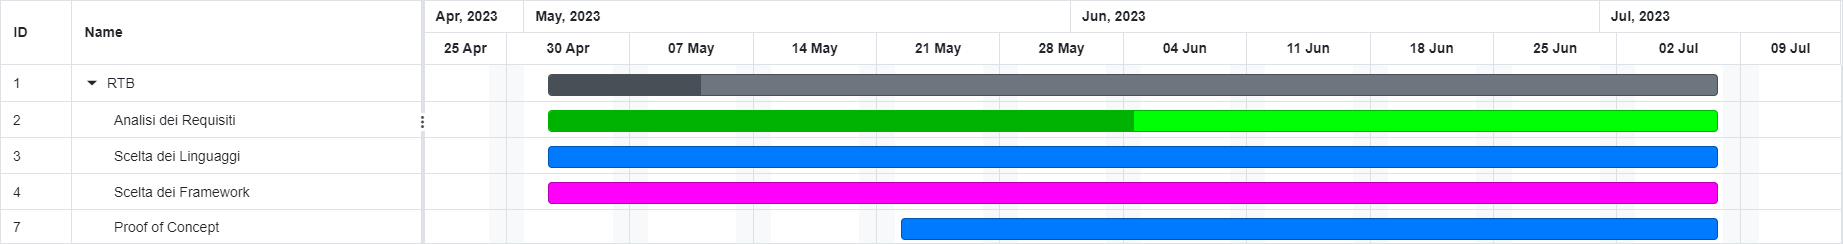
\includegraphics[scale=0.24]{RTB_2.png}\newline
\newline

\begin{center}
	\begin{tabularx}{\textwidth}{|X|X|X|X|}
		\hline
		\multicolumn{4}{|c|}{\textbf{Preventivo ore/costi}}                                      \\
		\hline
		\hline
		\textbf{Ruolo}  & \textbf{Costo orario (\euro)} & \textbf{Ore} & \textbf{Prezzo (\euro)} \\
		\hline
		Responsabile    & 30                            & 18(+6)       & 180                     \\
		\hline
		Amministratore  & 20                            & 17(+8)       & 160                     \\
		\hline
		Analista        & 25                            & 35(+14)      & 350                     \\
		\hline
		Progettista     & 25                            & 0(+0)        & 0                       \\
		\hline
		Programmatore   & 15                            & 0(+0)        & 0                       \\
		\hline
		Verificatore    & 15                            & 12(+4)       & 60                      \\
		\hline
		\hline
		\textbf{Totale} &                               & 82           & 1935                    \\
		\hline
	\end{tabularx}\\[8pt]
	\mbox{}\\
\end{center}

\begin{center}
	\begin{tabularx}{\textwidth}{|X|X|X|X|X|X|X|}
		\hline
		\multicolumn{7}{|c|}{\textbf{Preventivo ore per membro}}                                 \\
		\hline
		\hline
		\textbf{Membro}   & \textbf{Resp.}    & \textbf{Amm.}   & \textbf{Ana.} &
		\textbf{Proget.}  & \textbf{Program.} & \textbf{Verif.}                                  \\
		\hline
		Alberti Nicolas   & 6                 & 2               & 0             & 0 & 0 & 4(+4)  \\
		\hline
		Brotto Romina     & 0                 & 3               & 7(+7)         & 0 & 0 & 3      \\
		\hline
		Cavaliere Erica   & 0                 & 4(+4)           & 10            & 0 & 0 & 0      \\
		\hline
		Ceccato Francesco & 0                 & 0               & 12(+7)        & 0 & 0 & 0      \\
		\hline
		Salami Lorenzo    & 0                 & 4(+4)           & 6             & 0 & 0 & 5      \\
		\hline
		Soldà Matteo      & 12(+6)            & 2               & 0             & 0 & 0 & 0      \\
		\hline
		\hline
		\textbf{Totale}   & 18(+6)            & 17(+8)          & 35(+14)       & 0 & 0 & 12(+4) \\
		\hline
	\end{tabularx}\\[8pt]
	\mbox{}\\
\end{center}

\newpage

\subsubsection{Sprint 4}
\textbf{Data di inizio:} 17/05/2023\newline
\textbf{Data di fine:} 25/05/2023\newline
\newline
\textbf{Suddivisione del lavoro:}
\begin{itemize}
	\item incontro con il proponente per sistemare gli use case;
	\item inizio della stesura del \textit{Proof of Concept};
	\item decidere i linguaggi e i framework da utilizzare.
\end{itemize}
\textbf{Difficoltà incontrate:}
\begin{itemize}
	\item difficoltà nella decisione dei linguaggi da utilizzare, in quanto
	      ciascun membro del gruppo ha espresso preferenze ed opinioni diverse;
	\item difficoltà nell'interpretazione di alcuni Use Case, in particolare
	      nella definizione dei ruoli degli attori.
\end{itemize}
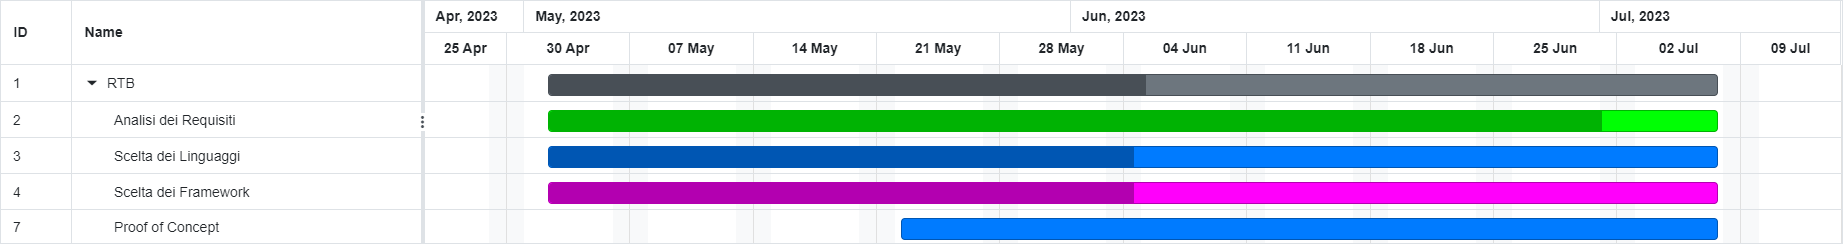
\includegraphics[scale=0.24]{RTB_3.png}\newline
\newline

\begin{center}
	\begin{tabularx}{\textwidth}{|X|X|X|X|}
		\hline
		\multicolumn{4}{|c|}{\textbf{Preventivo ore/costi}}                                      \\
		\hline
		\hline
		\textbf{Ruolo}  & \textbf{Costo orario (\euro)} & \textbf{Ore} & \textbf{Prezzo (\euro)} \\
		\hline
		Responsabile    & 30                            & 21(+3)       & 90                      \\
		\hline
		Amministratore  & 20                            & 21(+4)       & 80                      \\
		\hline
		Analista        & 25                            & 50(+15)      & 375                     \\
		\hline
		Progettista     & 25                            & 0(+0)        & 0                       \\
		\hline
		Programmatore   & 15                            & 0(+0)        & 0                       \\
		\hline
		Verificatore    & 15                            & 17(+5)       & 75                      \\
		\hline
		\hline
		\textbf{Totale} &                               & 109          & 2555                    \\
		\hline
	\end{tabularx}\\[8pt]
	\mbox{}\\
\end{center}

\begin{center}
	\begin{tabularx}{\textwidth}{|X|X|X|X|X|X|X|}
		\hline
		\multicolumn{7}{|c|}{\textbf{Preventivo ore per membro}}                                 \\
		\hline
		\hline
		\textbf{Membro}   & \textbf{Resp.}    & \textbf{Amm.}   & \textbf{Ana.} &
		\textbf{Proget.}  & \textbf{Program.} & \textbf{Verif.}                                  \\
		\hline
		Alberti Nicolas   & 6                 & 2               & 7(+7)         & 0 & 0 & 4      \\
		\hline
		Brotto Romina     & 3(+3)             & 3               & 7             & 0 & 0 & 3      \\
		\hline
		Cavaliere Erica   & 0                 & 6(+2)           & 10            & 0 & 0 & 0      \\
		\hline
		Ceccato Francesco & 0                 & 0               & 12            & 0 & 0 & 5(+5)  \\
		\hline
		Salami Lorenzo    & 0                 & 6(+2)           & 6             & 0 & 0 & 5      \\
		\hline
		Soldà Matteo      & 12                & 2               & 8(+8)         & 0 & 0 & 0      \\
		\hline
		\hline
		\textbf{Totale}   & 21(+3)            & 21(+4)          & 50(+15)       & 0 & 0 & 17(+5) \\
		\hline
	\end{tabularx}\\[8pt]
	\mbox{}\\
\end{center}

\newpage

\subsubsection{Sprint 5}
\textbf{Data di inizio:} 26/05/2023\newline
\textbf{Data di fine:} 02/06/2023\newline
\newline
\textbf{Suddivisione del lavoro:}
\begin{itemize}
	\item Incontro con il professor Cardin per discutere di alcuni dubbi sugli use case;
	\item Avanzamento del \textit{Proof of Concept};
	\item Aggiornamento dell'analisi dei requisiti.
\end{itemize}
\textbf{Difficoltà incontrate:}
\begin{itemize}
	\item Alcune difficoltà nella precisa definizione di alcuni sottocasi negli use case;
	\item Difficoltà nella comprensione del funzionamento di \textit{typescript} soprattutto nel dialogo tra client e server.
\end{itemize}
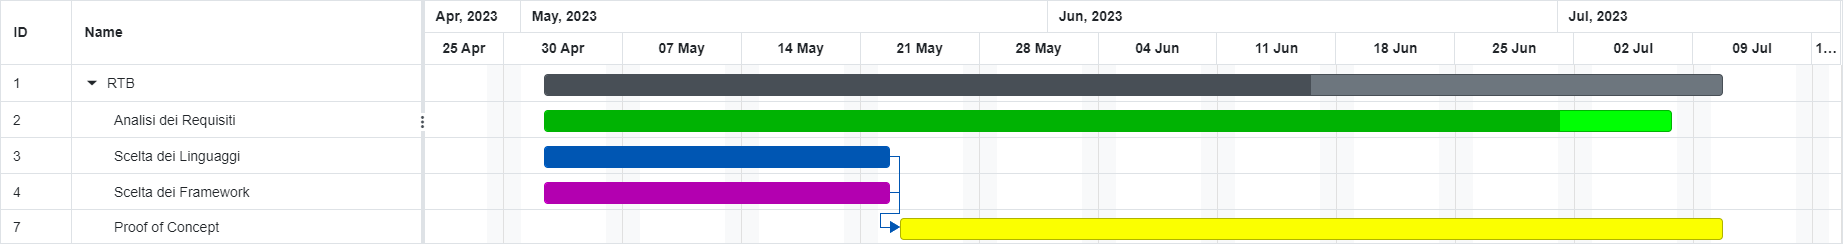
\includegraphics[scale=0.24]{RTB_4.png}\newline
\newline

\begin{center}
	\begin{tabularx}{\textwidth}{|X|X|X|X|}
		\hline
		\multicolumn{4}{|c|}{\textbf{Preventivo ore/costi}}                                      \\
		\hline
		\hline
		\textbf{Ruolo}  & \textbf{Costo orario (\euro)} & \textbf{Ore} & \textbf{Prezzo (\euro)} \\
		\hline
		Responsabile    & 30                            & 24(+3)       & 90                      \\
		\hline
		Amministratore  & 20                            & 23(+2)       & 40                      \\
		\hline
		Analista        & 25                            & 55(+5)       & 125                     \\
		\hline
		Progettista     & 25                            & 2(+2)        & 50                      \\
		\hline
		Programmatore   & 15                            & 1(+1)        & 15                      \\
		\hline
		Verificatore    & 15                            & 23(+6)       & 90                      \\
		\hline
		\hline
		\textbf{Totale} &                               & 128          & 2965                    \\
		\hline
	\end{tabularx}\\[8pt]
	\mbox{}\\
\end{center}

\begin{center}
	\begin{tabularx}{\textwidth}{|X|X|X|X|X|X|X|}
		\hline
		\multicolumn{7}{|c|}{\textbf{Preventivo ore per membro}}                                         \\
		\hline
		\hline
		\textbf{Membro}   & \textbf{Resp.}    & \textbf{Amm.}   & \textbf{Ana.} &
		\textbf{Proget.}  & \textbf{Program.} & \textbf{Verif.}                                          \\
		\hline
		Alberti Nicolas   & 6                 & 4(+2)           & 7             & 0     & 0     & 4      \\
		\hline
		Brotto Romina     & 3                 & 3               & 12(+5)        & 0     & 0     & 3      \\
		\hline
		Cavaliere Erica   & 3(+3)             & 6               & 10            & 0     & 0     & 0      \\
		\hline
		Ceccato Francesco & 0                 & 0               & 12            & 2(+2) & 0     & 5      \\
		\hline
		Salami Lorenzo    & 0                 & 6               & 6             & 0     & 0     & 11(+6) \\
		\hline
		Soldà Matteo      & 12                & 2               & 8             & 0     & 1(+1) & 0      \\
		\hline
		\hline
		\textbf{Totale}   & 24(+3)            & 23(+2)          & 55(+5)        & 2(+2) & 1(+1) & 23(+6) \\
		\hline
	\end{tabularx}\\[8pt]
	\mbox{}\\
\end{center}

\newpage

\subsubsection{Sprint 6}
\textbf{Data di inizio:} 03/06/2023\newline
\textbf{Data di fine:} 12/06/2023\newline
\newline
\textbf{Suddivisione del lavoro:}
\begin{itemize}
	\item Completare il \textit{Glossario} con eventuali termini mancanti;
	\item Chiedere al proponente un controllo dell'\textit{Analisi dei Requisiti};
	\item Avanzamento del \textit{Proof of Concept}.
\end{itemize}
\textbf{Difficoltà incontrate:}
\begin{itemize}
	\item Eseguire il \textit{Proof of Concept} nella macchina locale di ogni componente del gruppo, dovuto alla mancanza di alcuni pacchetti fondamentali per l'esecuzione del codice.
\end{itemize}
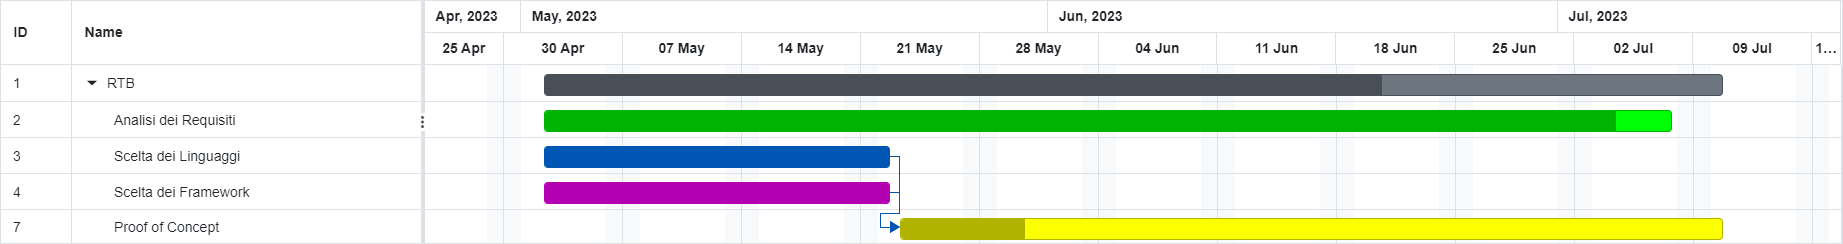
\includegraphics[scale=0.24]{RTB_5.png}\newline
\newline

\begin{center}
	\begin{tabularx}{\textwidth}{|X|X|X|X|}
		\hline
		\multicolumn{4}{|c|}{\textbf{Preventivo ore/costi}}                                      \\
		\hline
		\hline
		\textbf{Ruolo}  & \textbf{Costo orario (\euro)} & \textbf{Ore} & \textbf{Prezzo (\euro)} \\
		\hline
		Responsabile    & 30                            & 26(+2)       & 60                      \\
		\hline
		Amministratore  & 20                            & 24(+1)       & 20                      \\
		\hline
		Analista        & 25                            & 56(+1)       & 25                      \\
		\hline
		Progettista     & 25                            & 7(+5)        & 125                     \\
		\hline
		Programmatore   & 15                            & 16(+15)      & 225                     \\
		\hline
		Verificatore    & 15                            & 27(+4)       & 60                      \\
		\hline
		\hline
		\textbf{Totale} &                               & 156          & 3480                    \\
		\hline
	\end{tabularx}\\[8pt]
	\mbox{}\\
\end{center}

\begin{center}
	\begin{tabularx}{\textwidth}{|X|X|X|X|X|X|X|}
		\hline
		\multicolumn{7}{|c|}{\textbf{Preventivo ore per membro}}                                           \\
		\hline
		\hline
		\textbf{Membro}   & \textbf{Resp.}    & \textbf{Amm.}   & \textbf{Ana.} &
		\textbf{Proget.}  & \textbf{Program.} & \textbf{Verif.}                                            \\
		\hline
		Alberti Nicolas   & 8(+2)             & 4               & 7             & 0     & 0       & 4      \\
		\hline
		Brotto Romina     & 3                 & 4(+1)           & 12            & 0     & 0       & 3      \\
		\hline
		Cavaliere Erica   & 3                 & 6               & 10            & 0     & 0       & 4(+4)  \\
		\hline
		Ceccato Francesco & 0                 & 0               & 12            & 7(+5) & 0       & 5      \\
		\hline
		Salami Lorenzo    & 0                 & 6               & 7(+1)         & 0     & 0       & 11     \\
		\hline
		Soldà Matteo      & 12                & 2               & 8             & 0     & 16(+15) & 0      \\
		\hline
		\hline
		\textbf{Totale}   & 26(+2)            & 24(+1)          & 56(+1)        & 7(+5) & 16(+15) & 27(+4) \\
		\hline
	\end{tabularx}\\[8pt]
	\mbox{}\\
\end{center}

\newpage

\subsubsection{Sprint 7}
\textbf{Data di inizio:} 13/06/2023\newline
\textbf{Data di fine:} 19/06/2023\newline
\newline
\textbf{Suddivisione del lavoro:}
\begin{itemize}
	\item Avanzamento dello sviluppo del \textit{Proof of Concept}.
\end{itemize}
\textbf{Difficoltà incontrate:}
\begin{itemize}
	\item Eseguire correttamente il codice all'interno di un \textit{container Docker};
	\item Integrazione del database \textit{MongoDB} con il codice presente.
\end{itemize}
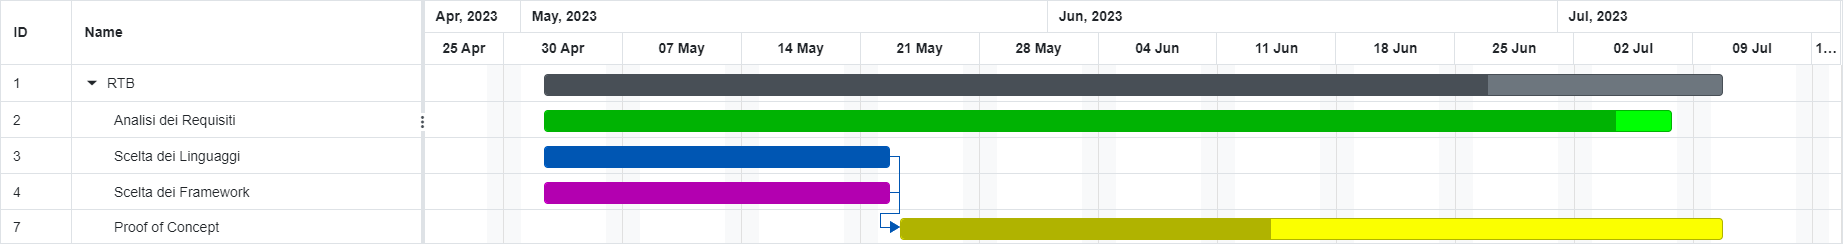
\includegraphics[scale=0.24]{RTB_6.png}\newline
\newline

\begin{center}
	\begin{tabularx}{\textwidth}{|X|X|X|X|}
		\hline
		\multicolumn{4}{|c|}{\textbf{Preventivo ore/costi}}                                      \\
		\hline
		\hline
		\textbf{Ruolo}  & \textbf{Costo orario (\euro)} & \textbf{Ore} & \textbf{Prezzo (\euro)} \\
		\hline
		Responsabile    & 30                            & 29(+3)       & 90                      \\
		\hline
		Amministratore  & 20                            & 26(+2)       & 40                      \\
		\hline
		Analista        & 25                            & 57(+1)       & 25                      \\
		\hline
		Progettista     & 25                            & 11(+4)       & 100                     \\
		\hline
		Programmatore   & 15                            & 26(+10)      & 150                     \\
		\hline
		Verificatore    & 15                            & 31(+4)       & 60                      \\
		\hline
		\hline
		\textbf{Totale} &                               & 180          & 3945                    \\
		\hline
	\end{tabularx}\\[8pt]
	\mbox{}\\
\end{center}

\begin{center}
	\begin{tabularx}{\textwidth}{|X|X|X|X|X|X|X|}
		\hline
		\multicolumn{7}{|c|}{\textbf{Preventivo ore per membro}}                                            \\
		\hline
		\hline
		\textbf{Membro}   & \textbf{Resp.}    & \textbf{Amm.}   & \textbf{Ana.} &
		\textbf{Proget.}  & \textbf{Program.} & \textbf{Verif.}                                             \\
		\hline
		Alberti Nicolas   & 8                 & 4               & 7             & 4(+4)  & 0       & 4      \\
		\hline
		Brotto Romina     & 3                 & 6(+2)           & 12            & 0      & 0       & 3      \\
		\hline
		Cavaliere Erica   & 3                 & 6               & 10            & 0      & 10(+10) & 4      \\
		\hline
		Ceccato Francesco & 0                 & 0               & 12            & 7      & 0       & 9(+4)  \\
		\hline
		Salami Lorenzo    & 3(+3)             & 6               & 7             & 0      & 0       & 11     \\
		\hline
		Soldà Matteo      & 12                & 2               & 9(+1)         & 0      & 16      & 0      \\
		\hline
		\hline
		\textbf{Totale}   & 29(+3)            & 26(+2)          & 57(+1)        & 11(+4) & 26(+10) & 31(+4) \\
		\hline
	\end{tabularx}\\[8pt]
	\mbox{}\\
\end{center}

\newpage


\subsubsection{Sprint 8}
\textbf{Data di inizio:} 19/06/2023\newline
\textbf{Data di fine:} 03/07/2023\newline
\newline
\textbf{Suddivisione del lavoro:}
\begin{itemize}
	\item Avanzamento dello sviluppo del \textit{Proof of Concept}
	      \begin{itemize}
		      \item Implementazione del MongoDB e primo collegamento al server;
		      \item Implementazione modello sensore;
		      \item Implementazione modello area illuminata
	      \end{itemize}
\end{itemize}
\textbf{Difficoltà incontrate:}
\begin{itemize}
	\item Eseguire correttamente il codice all'interno di un \textit{container Docker};
	\item Integrazione del database \textit{MongoDB} con il codice presente.
\end{itemize}
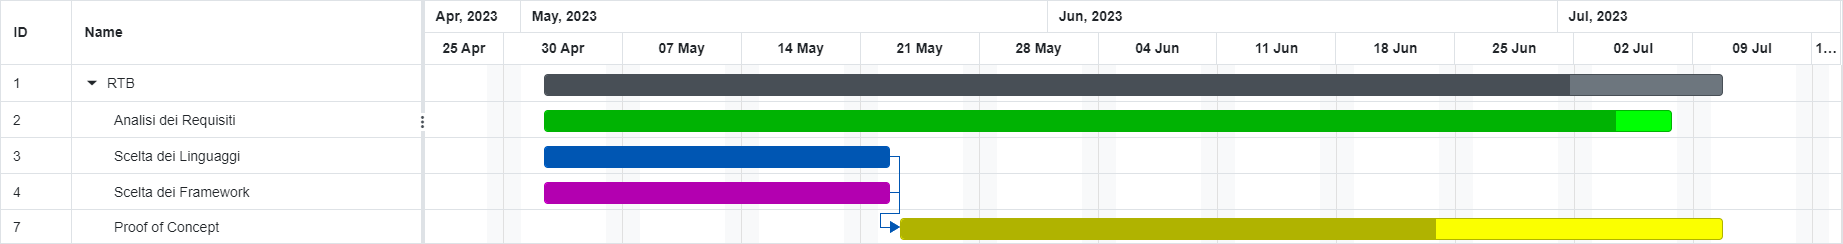
\includegraphics[scale=0.24]{RTB_7.png}\newline
\newline

\begin{center}
	\begin{tabularx}{\textwidth}{|X|X|X|X|}
		\hline
		\multicolumn{4}{|c|}{\textbf{Preventivo ore/costi}}                                      \\
		\hline
		\hline
		\textbf{Ruolo}  & \textbf{Costo orario (\euro)} & \textbf{Ore} & \textbf{Prezzo (\euro)} \\
		\hline
		Responsabile    & 30                            & 30(+1)       & 30                      \\
		\hline
		Amministratore  & 20                            & 28(+2)       & 40                      \\
		\hline
		Analista        & 25                            & 59(+2)       & 50                      \\
		\hline
		Progettista     & 25                            & 18(+7)       & 175                     \\
		\hline
		Programmatore   & 15                            & 36(+10)      & 150                     \\
		\hline
		Verificatore    & 15                            & 36(+5)       & 75                      \\
		\hline
		\hline
		\textbf{Totale} &                               & 207          & 4465                    \\
		\hline
	\end{tabularx}\\[8pt]
	\mbox{}\\
\end{center}

\begin{center}
	\begin{tabularx}{\textwidth}{|X|X|X|X|X|X|X|}
		\hline
		\multicolumn{7}{|c|}{\textbf{Preventivo ore per membro}}                                            \\
		\hline
		\hline
		\textbf{Membro}   & \textbf{Resp.}    & \textbf{Amm.}   & \textbf{Ana.} &
		\textbf{Proget.}  & \textbf{Program.} & \textbf{Verif.}                                             \\
		\hline
		Alberti Nicolas   & 8                 & 4               & 7             & 4      & 10(+10) & 4      \\
		\hline
		Brotto Romina     & 3                 & 8(+2)           & 12            & 0      & 0       & 3      \\
		\hline
		Cavaliere Erica   & 3                 & 6               & 10            & 7(+7)  & 10      & 4      \\
		\hline
		Ceccato Francesco & 0                 & 0               & 14(+2)        & 7      & 0       & 9      \\
		\hline
		Salami Lorenzo    & 4(+1)             & 6               & 7             & 0      & 0       & 11     \\
		\hline
		Soldà Matteo      & 12                & 2               & 9             & 0      & 16      & 5(+5)  \\
		\hline
		\hline
		\textbf{Totale}   & 30(+1)            & 28(+2)          & 59(+2)        & 18(+7) & 36(+10) & 36(+5) \\
		\hline
	\end{tabularx}\\[8pt]
	\mbox{}\\
\end{center}

\newpage

\subsubsection{Sprint 9}
\textbf{Data di inizio:} 04/07/2023\newline
\textbf{Data di fine:} 11/07/2023\newline
\newline
\textbf{Suddivisione del lavoro:}
\begin{itemize}
	\item Avanzamento dello sviluppo del \textit{Proof of Concept}
	      \begin{itemize}
		      \item Sistemazione conflitti dovuti all'integrazione sul branch \textit{dev};
		      \item Integrazione del DB nel branch \textit{dev};
		      \item Pulizia delle \textit{issues} legate agli avanzamenti nel \textit{Proof of Concept}.
	      \end{itemize}
\end{itemize}
\textbf{Difficoltà incontrate:}
\begin{itemize}
	\item Risoluzione dei conflitti di \textit{merge}.
\end{itemize}
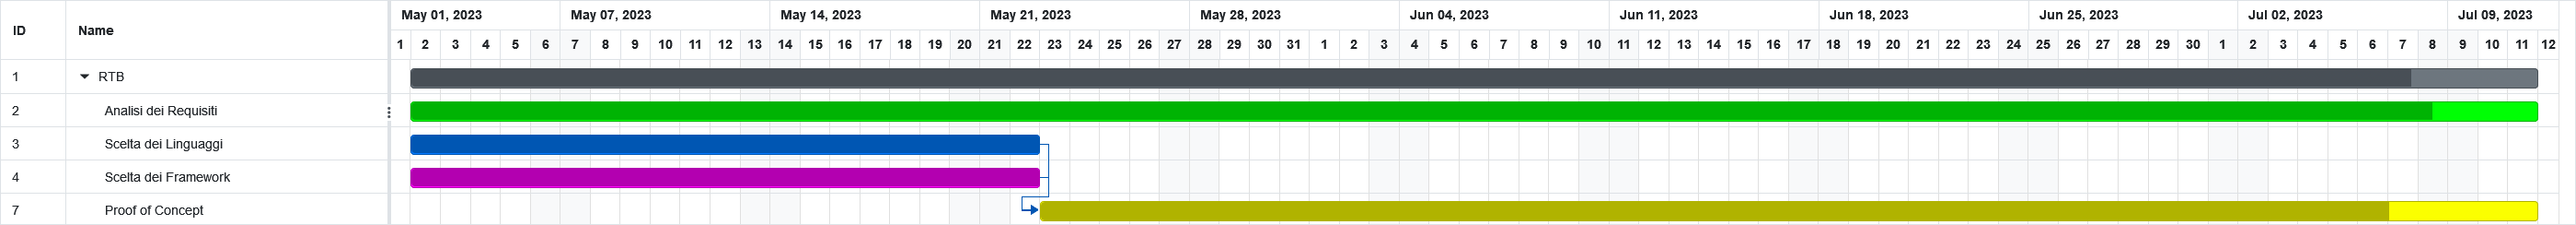
\includegraphics[scale=0.176]{RTB_8.png}\newline
\newline
\begin{center}
	\begin{tabularx}{\textwidth}{|X|X|X|X|}
		\hline
		\multicolumn{4}{|c|}{\textbf{Preventivo ore/costi}}                                      \\
		\hline
		\hline
		\textbf{Ruolo}  & \textbf{Costo orario (\euro)} & \textbf{Ore} & \textbf{Prezzo (\euro)} \\
		\hline
		Responsabile    & 30                            & 31(+1)       & 30                      \\
		\hline
		Amministratore  & 20                            & 30(+2)       & 40                      \\
		\hline
		Analista        & 25                            & 61(+2)       & 50                      \\
		\hline
		Progettista     & 25                            & 25(+7)       & 175                     \\
		\hline
		Programmatore   & 15                            & 46(+10)      & 150                     \\
		\hline
		Verificatore    & 15                            & 41(+5)       & 75                      \\
		\hline
		\hline
		\textbf{Totale} &                               & 234          & 4985                    \\
		\hline
	\end{tabularx}\\[8pt]
	\mbox{}\\
\end{center}

\begin{center}
	\begin{tabularx}{\textwidth}{|X|X|X|X|X|X|X|}
		\hline
		\multicolumn{7}{|c|}{\textbf{Preventivo ore per membro}}                                            \\
		\hline
		\hline
		\textbf{Membro}   & \textbf{Resp.}    & \textbf{Amm.}   & \textbf{Ana.} &
		\textbf{Proget.}  & \textbf{Program.} & \textbf{Verif.}                                             \\
		\hline
		Alberti Nicolas   & 8                 & 4               & 9(+2)         & 4      & 10      & 4      \\
		\hline
		Brotto Romina     & 3                 & 8               & 12            & 0      & 0       & 8(+5)  \\
		\hline
		Cavaliere Erica   & 3                 & 8(+2)           & 10            & 7      & 10      & 4      \\
		\hline
		Ceccato Francesco & 1(+1)             & 0               & 14            & 7      & 0       & 9      \\
		\hline
		Salami Lorenzo    & 4                 & 6               & 7             & 0      & 10(+10) & 11     \\
		\hline
		Soldà Matteo      & 12                & 2               & 9             & 7(+7)  & 16      & 5      \\
		\hline
		\hline
		\textbf{Totale}   & 31(+1)            & 30(+2)          & 61(+2)        & 25(+7) & 46(+10) & 41(+5) \\
		\hline
	\end{tabularx}\\[8pt]
	\mbox{}\\
\end{center}

\newpage

\subsubsection{Sprint 10}
\textbf{Data di inizio:} 12/07/2023\newline
\textbf{Data di fine:} 19/07/2023\newline
\newline
\textbf{Suddivisione del lavoro:}
\begin{itemize}
	\item Avanzamento dello sviluppo del \textit{Proof of Concept}
	      \begin{itemize}
		      \item Completata la parte legata alla modifica di un'area illuminata;
		      \item Aggiunte le possibilità di inserimento, modifica ed eliminazione
		            di sensori, lampioni ed aree illuminate;
		      \item Integrazione della segnalazione dei guasti.
	      \end{itemize}
\end{itemize}
\textbf{Difficoltà incontrate:}
\begin{itemize}
	\item Nulla da segnalare.
\end{itemize}
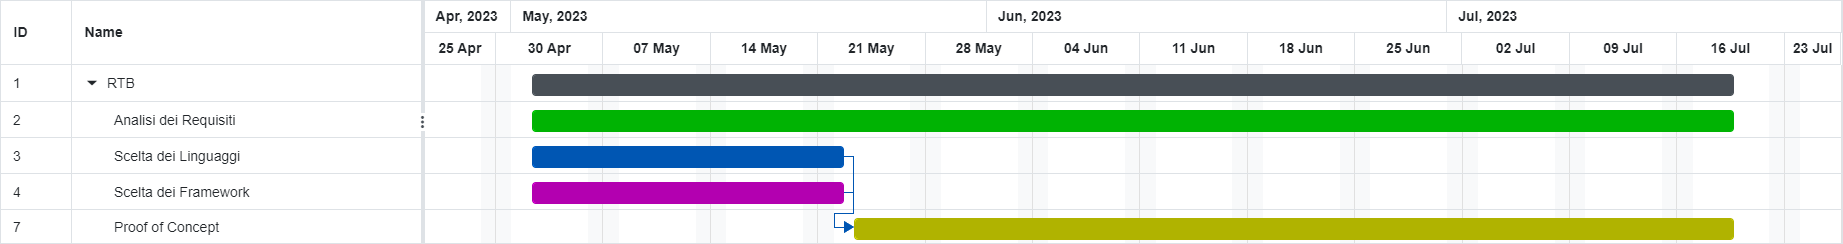
\includegraphics[scale=0.178]{RTB_9.png}\newline
\newline
\begin{center}
	\begin{tabularx}{\textwidth}{|X|X|X|X|}
		\hline
		\multicolumn{4}{|c|}{\textbf{Preventivo ore/costi}}                                      \\
		\hline
		\hline
		\textbf{Ruolo}  & \textbf{Costo orario (\euro)} & \textbf{Ore} & \textbf{Prezzo (\euro)} \\
		\hline
		Responsabile    & 30                            & 32(+1)       & 30                      \\
		\hline
		Amministratore  & 20                            & 32(+2)       & 40                      \\
		\hline
		Analista        & 25                            & 62(+1)       & 25                      \\
		\hline
		Progettista     & 25                            & 31(+6)       & 150                     \\
		\hline
		Programmatore   & 15                            & 56(+10)      & 150                     \\
		\hline
		Verificatore    & 15                            & 46(+5)       & 75                      \\
		\hline
		\hline
		\textbf{Totale} &                               & 259          & 5455                    \\
		\hline
	\end{tabularx}\\[8pt]
	\mbox{}\\
\end{center}

\begin{center}
	\begin{tabularx}{\textwidth}{|X|X|X|X|X|X|X|}
		\hline
		\multicolumn{7}{|c|}{\textbf{Preventivo ore per membro}}                                            \\
		\hline
		\hline
		\textbf{Membro}   & \textbf{Resp.}    & \textbf{Amm.}   & \textbf{Ana.} &
		\textbf{Proget.}  & \textbf{Program.} & \textbf{Verif.}                                             \\
		\hline
		Alberti Nicolas   & 8                 & 4               & 10(+1)        & 4      & 10      & 4      \\
		\hline
		Brotto Romina     & 3                 & 8               & 12            & 0      & 5(+5)   & 8      \\
		\hline
		Cavaliere Erica   & 3                 & 8               & 10            & 7      & 10      & 9(+5)  \\
		\hline
		Ceccato Francesco & 1                 & 2(+2)           & 14            & 7      & 5(+5)   & 9      \\
		\hline
		Salami Lorenzo    & 4                 & 6               & 7             & 6(+6)  & 10      & 11     \\
		\hline
		Soldà Matteo      & 13(+1)            & 2               & 9             & 7      & 16      & 5      \\
		\hline
		\hline
		\textbf{Totale}   & 32(+1)            & 32(+2)          & 62(+1)        & 31(+6) & 56(+10) & 46(+5) \\
		\hline
	\end{tabularx}\\[8pt]
	\mbox{}\\
\end{center}

\newpage

\subsubsection{Sprint 11}
\textbf{Data di inizio:} 20/07/2023\newline
\textbf{Data di fine:} 31/07/2023\newline
\newline
\textbf{Suddivisione del lavoro:}
\begin{itemize}
	\item Allineamento e controllo documentazione in vista della revisione RTB.
	      \begin{itemize}
		      \item Revisionati tutti i documenti per la \textit{RTB};
		      \item Approvate le versioni finali.
	      \end{itemize}
\end{itemize}
\textbf{Difficoltà incontrate:}
\begin{itemize}
	\item Nulla da segnalare.
\end{itemize}
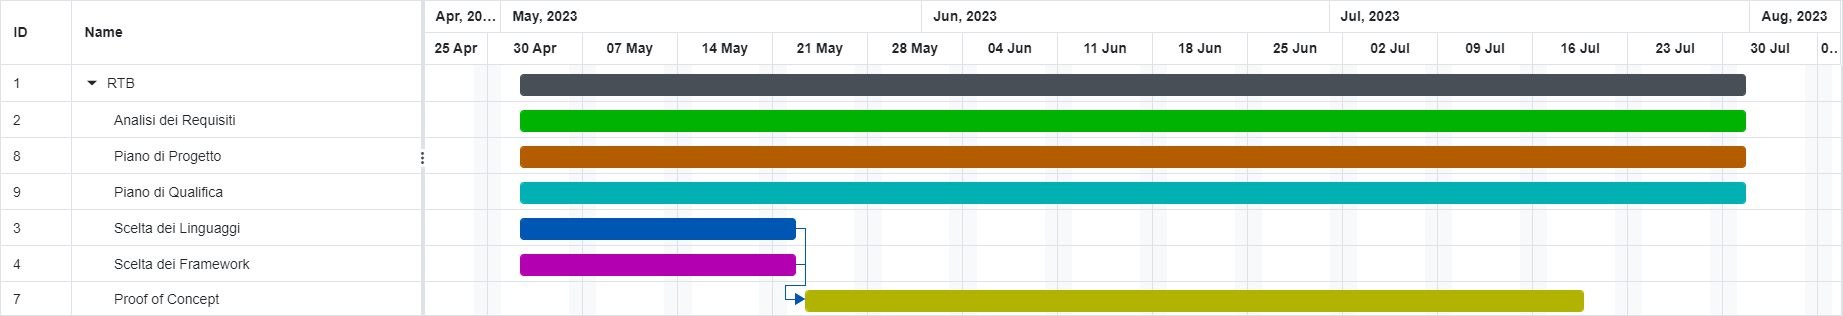
\includegraphics[scale=0.178]{RTB_10e11.png}\newline
\newline
\begin{center}
	\begin{tabularx}{\textwidth}{|X|X|X|X|}
		\hline
		\multicolumn{4}{|c|}{\textbf{Preventivo ore/costi}}                                      \\
		\hline
		\hline
		\textbf{Ruolo}  & \textbf{Costo orario (\euro)} & \textbf{Ore} & \textbf{Prezzo (\euro)} \\
		\hline
		Responsabile    & 30                            & 34(+2)       & 60                      \\
		\hline
		Amministratore  & 20                            & 35(+3)       & 60                      \\
		\hline
		Analista        & 25                            & 70(+8)       & 200                     \\
		\hline
		Progettista     & 25                            & 31(+0)       & 0                       \\
		\hline
		Programmatore   & 15                            & 56(+0)       & 0                       \\
		\hline
		Verificatore    & 15                            & 56(+10)      & 150                     \\
		\hline
		\hline
		\textbf{Totale} &                               & 282          & 5925                    \\
		\hline
	\end{tabularx}\\[8pt]
	\mbox{}\\
\end{center}

\begin{center}
	\begin{tabularx}{\textwidth}{|X|X|X|X|X|X|X|}
		\hline
		\multicolumn{7}{|c|}{\textbf{Preventivo ore per membro}}                                            \\
		\hline
		\hline
		\textbf{Membro}   & \textbf{Resp.}    & \textbf{Amm.}   & \textbf{Ana.} &
		\textbf{Proget.}  & \textbf{Program.} & \textbf{Verif.}                                             \\
		\hline
		Alberti Nicolas   & 9(+1)             & 4               & 10            & 4      & 10     & 6(+2)   \\
		\hline
		Brotto Romina     & 3                 & 9(+1)           & 14(+2)        & 0      & 5      & 10(+2)  \\
		\hline
		Cavaliere Erica   & 3                 & 10(+2)          & 12(+2)        & 7      & 10     & 11(+2)  \\
		\hline
		Ceccato Francesco & 1                 & 2               & 16(+2)        & 7      & 5      & 11(+2)  \\
		\hline
		Salami Lorenzo    & 4                 & 6               & 9(+2)         & 6      & 10     & 11      \\
		\hline
		Soldà Matteo      & 14(+1)            & 2               & 9             & 7      & 16     & 7(+2)   \\
		\hline
		\hline
		\textbf{Totale}   & 34(+2)            & 35(+3)          & 70(+8)        & 31(+0) & 56(+0) & 56(+10) \\
		\hline
	\end{tabularx}\\[8pt]
	\mbox{}\\
\end{center}

\newpage

\subsubsection{Sprint 12}
\textbf{Data di inizio:} 01/08/2023\newline
\textbf{Data di fine:} 11/08/2023\newline
\newline
\textbf{Suddivisione del lavoro:}
\begin{itemize}
	\item Allineamento e controllo documentazione in vista della seconda parte di revisione RTB.
	      \begin{itemize}
		      \item Sistemazione dei documenti per cui c'era necessità di fix;
		      \item Approvate le versioni finali.
	      \end{itemize}
\end{itemize}
\textbf{Difficoltà incontrate:}
\begin{itemize}
	\item Nulla da segnalare.
\end{itemize}
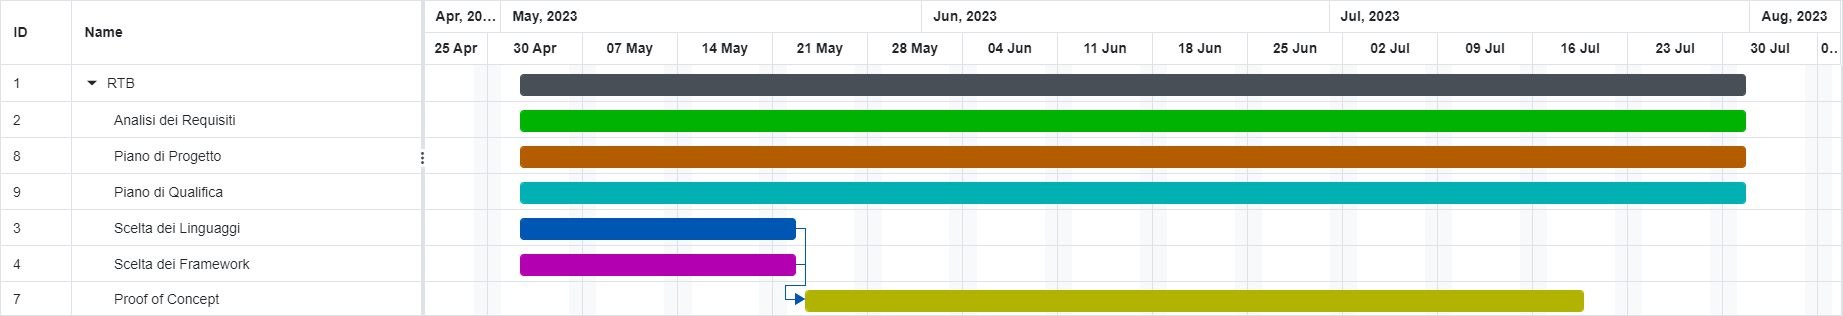
\includegraphics[scale=0.178]{RTB_10e11.png}\newline
\newline
\begin{center}
	\begin{tabularx}{\textwidth}{|X|X|X|X|}
		\hline
		\multicolumn{4}{|c|}{\textbf{Preventivo ore/costi}}                                      \\
		\hline
		\hline
		\textbf{Ruolo}  & \textbf{Costo orario (\euro)} & \textbf{Ore} & \textbf{Prezzo (\euro)} \\
		\hline
		Responsabile    & 30                            & 35(+1)       & 30                      \\
		\hline
		Amministratore  & 20                            & 37(+2)       & 40                      \\
		\hline
		Analista        & 25                            & 75(+5)       & 125                     \\
		\hline
		Progettista     & 25                            & 31(+0)       & 0                       \\
		\hline
		Programmatore   & 15                            & 56(+0)       & 0                       \\
		\hline
		Verificatore    & 15                            & 61(+5)       & 75                      \\
		\hline
		\hline
		\textbf{Totale} &                               & 295          & 6195                    \\
		\hline
	\end{tabularx}\\[8pt]
	\mbox{}\\
\end{center}

\begin{center}
	\begin{tabularx}{\textwidth}{|X|X|X|X|X|X|X|}
		\hline
		\multicolumn{7}{|c|}{\textbf{Preventivo ore per membro}}                                           \\
		\hline
		\hline
		\textbf{Membro}   & \textbf{Resp.}    & \textbf{Amm.}   & \textbf{Ana.} &
		\textbf{Proget.}  & \textbf{Program.} & \textbf{Verif.}                                            \\
		\hline
		Alberti Nicolas   & 9                 & 4               & 11(+1)        & 4      & 10     & 6      \\
		\hline
		Brotto Romina     & 3                 & 10(+1)          & 14            & 0      & 5      & 12(+2) \\
		\hline
		Cavaliere Erica   & 4(+1)             & 11(+1)          & 12            & 7      & 10     & 11(+2) \\
		\hline
		Ceccato Francesco & 1                 & 2               & 17(+1)        & 7      & 5      & 11     \\
		\hline
		Salami Lorenzo    & 4                 & 6               & 11(+2)        & 6      & 10     & 11     \\
		\hline
		Soldà Matteo      & 14                & 2               & 10(+1)        & 7      & 16     & 8(+1)  \\
		\hline
		\hline
		\textbf{Totale}   & 35(+1)            & 37(+2)          & 75(+5)        & 31(+0) & 56(+0) & 61(+5) \\
		\hline
	\end{tabularx}\\[8pt]
	\mbox{}\\
\end{center}

\newpage

\subsubsection{Sprint 13}
\textbf{Data di inizio:} 12/08/2023\newline
\textbf{Data di fine:} 21/08/2023\newline
\newline
\textbf{Suddivisione del lavoro:}
\begin{itemize}
	\item Analisi della valutazione \textit{RTB}
	      \begin{itemize}
		      \item Creazione issues per sistemare i punti critici;
		      \item Creazione issues per procedere con lo sviluppo del codice.
	      \end{itemize}
\end{itemize}
\textbf{Difficoltà incontrate:}
\begin{itemize}
	\item Nulla da segnalare.
\end{itemize}
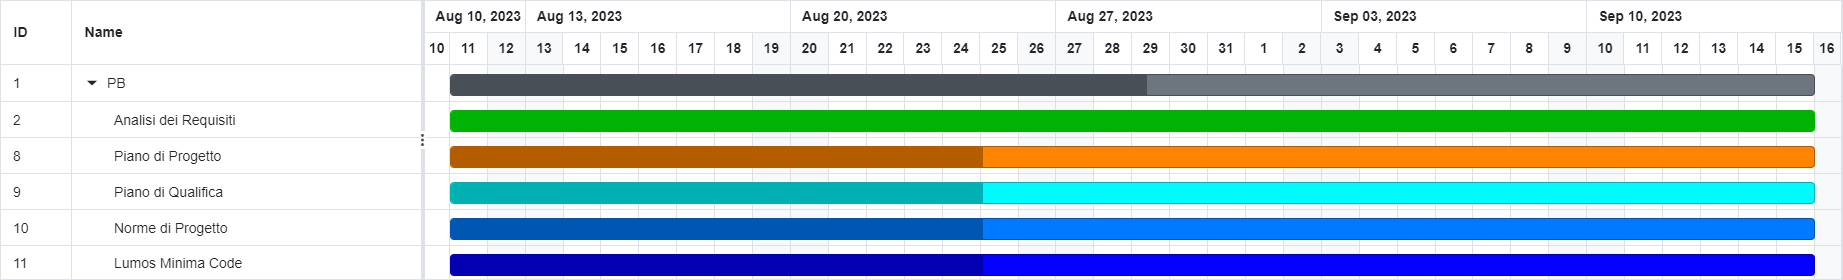
\includegraphics[scale=0.178]{PB_1.png}\newline
\newline
\begin{center}
	\begin{tabularx}{\textwidth}{|X|X|X|X|}
		\hline
		\multicolumn{4}{|c|}{\textbf{Preventivo ore/costi}}                                      \\
		\hline
		\hline
		\textbf{Ruolo}  & \textbf{Costo orario (\euro)} & \textbf{Ore} & \textbf{Prezzo (\euro)} \\
		\hline
		Responsabile    & 30                            & 37(+2)       & 60                      \\
		\hline
		Amministratore  & 20                            & 39(+2)       & 40                      \\
		\hline
		Analista        & 25                            & 80(+5)       & 125                     \\
		\hline
		Progettista     & 25                            & 36(+5)       & 125                     \\
		\hline
		Programmatore   & 15                            & 66(+10)      & 150                     \\
		\hline
		Verificatore    & 15                            & 65(+4)       & 60                      \\
		\hline
		\hline
		\textbf{Totale} &                               & 323          & 6755                    \\
		\hline
	\end{tabularx}\\[8pt]
	\mbox{}\\
\end{center}

\begin{center}
	\begin{tabularx}{\textwidth}{|X|X|X|X|X|X|X|}
		\hline
		\multicolumn{7}{|c|}{\textbf{Preventivo ore per membro}}                                            \\
		\hline
		\hline
		\textbf{Membro}   & \textbf{Resp.}    & \textbf{Amm.}   & \textbf{Ana.} &
		\textbf{Proget.}  & \textbf{Program.} & \textbf{Verif.}                                             \\
		\hline
		Alberti Nicolas   & 9                 & 4               & 11            & 6(+2)  & 13(+3)  & 6      \\
		\hline
		Brotto Romina     & 4(+1)            & 10              & 16(+2)        & 0      & 5       & 14(+2) \\
		\hline
		Cavaliere Erica   & 4                 & 12(+1)          & 12            & 9(+2)  & 11(+1)  & 11     \\
		\hline
		Ceccato Francesco & 2(+1)             & 2               & 17            & 8(+1)  & 6(+1)   & 11     \\
		\hline
		Salami Lorenzo    & 4                 & 6               & 11            & 9(+3)  & 10      & 12(+1) \\
		\hline
		Soldà Matteo      & 14                & 3(+1)           & 10            & 7      & 20(+4)  & 9(+1)  \\
		\hline
		\hline
		\textbf{Totale}   & 37(+2)            & 39(+2)          & 80(+5)        & 36(+5) & 66(+10) & 65(+4) \\
		\hline
	\end{tabularx}\\[8pt]
	\mbox{}\\
\end{center}

\newpage

\subsubsection{Sprint 14}
\textbf{Data di inizio:} 21/08/2023\newline
\textbf{Data di fine:} 31/08/2023\newline
\newline
\textbf{Suddivisione del lavoro:}
\begin{itemize}
	\item Erica si occupa di spostare i documenti nelle cartelle corrette, quali verbali e lettera di presentazione;
	\item Romina si occupa di aggiornare il Piano di Progetto;
	\item Lorenzo provvedera` ad aggiornare e modificare il Piano di Qualifica;
	\item Nicolas provvedera` a redigere una versione di base della Specifica Architetturale e della Specifica Tecnica.
	\item Matteo si occupera` dell’implementazione della modifica della luminosita` temporizzata per le aree illuminate
	\item Erica e Francesco procederanno con gli unit test;
	\item Matteo e Francesco si occuperanno del meccanismo di login.
\end{itemize}
\textbf{Difficoltà incontrate:}
\begin{itemize}
	\item Limitazione della visualizzazione delle pagine in base al ruolo
	\item Implementazione totale degli unit-test.
	\item Implementazione totale dei test
\end{itemize}
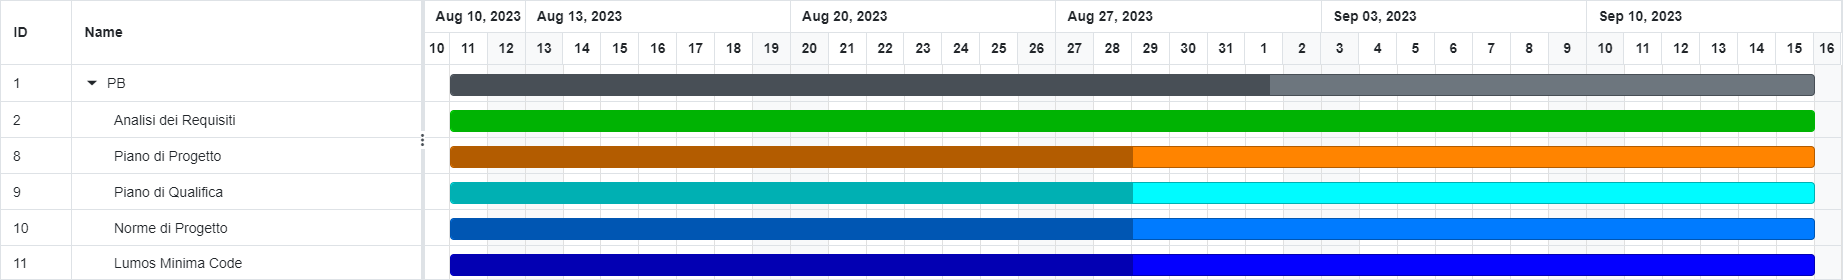
\includegraphics[scale=0.178]{PB_2.png}\newline
\newline
\begin{center}
	\begin{tabularx}{\textwidth}{|X|X|X|X|}
		\hline
		\multicolumn{4}{|c|}{\textbf{Preventivo ore/costi}}                                      \\
		\hline
		\hline
		\textbf{Ruolo}  & \textbf{Costo orario (\euro)} & \textbf{Ore} & \textbf{Prezzo (\euro)} \\
		\hline
		Responsabile    & 30                            & 49(+12)       & 360                      \\
		\hline
		Amministratore  & 20                            & 42(+3)       & 60                      \\
		\hline
		Analista        & 25                            & 90(+10)       & 250                     \\
		\hline
		Progettista     & 25                            & 86(+50)       & 1250                     \\
		\hline
		Programmatore   & 15                            & 86(+20)      & 300                    \\
		\hline
		Verificatore    & 15                            & 70(+5)       & 75                      \\
		\hline
		\hline
		\textbf{Totale} &                               & 423          & 9050                    \\
		\hline
	\end{tabularx}\\[8pt]
	\mbox{}\\
\end{center}

\begin{center}
	\begin{tabularx}{\textwidth}{|X|X|X|X|X|X|X|}
		\hline
		\multicolumn{7}{|c|}{\textbf{Preventivo ore per membro}}                                            \\
		\hline
		\hline
		\textbf{Membro}   & \textbf{Resp.}    & \textbf{Amm.}   & \textbf{Ana.} &
		\textbf{Proget.}  & \textbf{Program.} & \textbf{Verif.}                                             \\
		\hline
		Alberti Nicolas   & 9                 & 4               & 11            & 16(+10)  		& 18(+5) 	 & 8(+2)      \\
		\hline
		Brotto Romina     & 8(+4)                & 10              & 17(+1)        & 20(+20)      & 5       & 14 \\
		\hline
		Cavaliere Erica   & 8(+4)                & 12             & 15(+3)         & 9 		 & 16(+5) 	 & 11     \\
		\hline
		Ceccato Francesco & 2                & 5(+3)            & 17            & 13 (+5) 		& 16(+10)  	& 11     \\
		\hline
		Salami Lorenzo    & 8(+4)                & 6               & 14(+3)      & 14 (+5)		 & 10      & 12 \\
		\hline
		Soldà Matteo      & 14                & 3           & 13(+3)            & 17 (+10)    	 & 20 	& 12(+3)  \\
		\hline
		\hline
		\textbf{Totale}   & 49(+12)            & 42(+3)          & 90(+10)        & 86(+50)  & 86(+20) & 70(+5) \\
		\hline
	\end{tabularx}\\[8pt]
	\mbox{}\\
\end{center}

\newpage

\subsubsection{Sprint 15}
\textbf{Data di inizio:} 01/09/2023\newline
\textbf{Data di fine:} 10/09/2023\newline
\newline
\textbf{Suddivisione del lavoro:}
\begin{itemize}
	\item Romina si occupa di aggiornare le Norme di Progetto
	\item Lorenzo ultimera` il Piano di Qualifica 
	\item Nicolas si occupera` di stendere una versione di base della Specifica Architetturale e della Specifica Tecnica
	\item Matteo si occupera` di implementare la modifica della luminosita` temporizzata per le aree illuminate
	\item Erica e Francesco procederanno con gli unit test
\end{itemize}
\textbf{Difficoltà incontrate:}
\begin{itemize}
	\item Implementazione layout responsive
	\item Implementazione totale dei test.
\end{itemize}
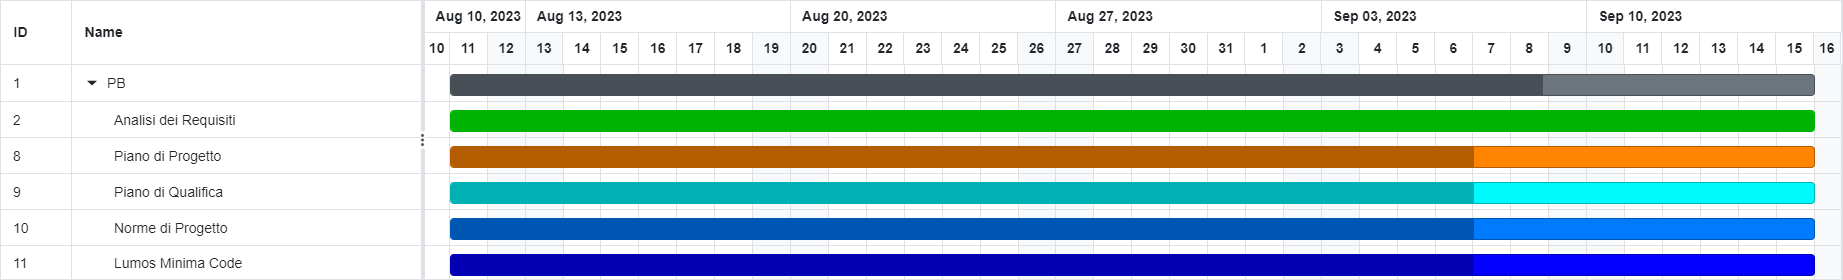
\includegraphics[scale=0.178]{PB_3.png}\newline
\newline
\begin{center}
	\begin{tabularx}{\textwidth}{|X|X|X|X|}
		\hline
		\multicolumn{4}{|c|}{\textbf{Preventivo ore/costi}}                                      \\
		\hline
		\hline
		\textbf{Ruolo}  & \textbf{Costo orario (\euro)} & \textbf{Ore} & \textbf{Prezzo (\euro)} \\
		\hline
		Responsabile    & 30                            & 61(+12)       & 360                      \\
		\hline
		Amministratore  & 20                            & 45(+3)       & 60                      \\
		\hline
		Analista        & 25                            & 100(+10)       & 250                     \\
		\hline
		Progettista     & 25                            & 131(+45)       & 1125                     \\
		\hline
		Programmatore   & 15                            & 106(+20)      & 300                    \\
		\hline
		Verificatore    & 15                            & 80(+10)       & 150                      \\
		\hline
		\hline
		\textbf{Totale} &                               & 523          & 11295                    \\
		\hline
	\end{tabularx}\\[8pt]
	\mbox{}\\
\end{center}

\begin{center}
	\begin{tabularx}{\textwidth}{|X|X|X|X|X|X|X|}
		\hline
		\multicolumn{7}{|c|}{\textbf{Preventivo ore per membro}}                                            \\
		\hline
		\hline
		\textbf{Membro}   & \textbf{Resp.}    & \textbf{Amm.}   & \textbf{Ana.} &
		\textbf{Proget.}  & \textbf{Program.} & \textbf{Verif.}                                             \\
		\hline
		Alberti Nicolas   & 9                 & 4               & 15(+4)            & 23(+7)  		& 18 		 & 12(+4)      \\
		\hline
		Brotto Romina     & 8                & 10              & 17       		& 23(+3)    	 & 15(+10)       & 14 \\
		\hline
		Cavaliere Erica   & 10(+2)                & 12             & 17(+2)        & 21(+12) 		 & 19(+3)	 	 & 14(+3)     \\
		\hline
		Ceccato Francesco & 10(+8)                & 5            & 17            & 22(+9) 		& 18(+2) 			& 14(+3)     \\
		\hline
		Salami Lorenzo    & 10(+2)                & 6               & 16(+2)      & 23(+9) 		 & 15(+5)    	  & 12 \\
		\hline
		Soldà Matteo      & 14                & 6(+3)           & 15(+2)           & 22(+5)    	 & 20 		& 12  \\
		\hline
		\hline
		\textbf{Totale}   & 61(+12)            & 45(+3)          & 100(+10)        & 131(+45)  & 106(+20) & 80(+10) \\
		\hline
	\end{tabularx}\\[8pt]
	\mbox{}\\
\end{center}

\newpage

\subsubsection{Sprint 16}
\textbf{Data di inizio:} 11/09/2023\newline
\textbf{Data di fine:} 20/09/2023\newline
\newline
\textbf{Suddivisione del lavoro:}
\begin{itemize}
	\item Romina aggiornerà il Piano di Progetto allo sprint corrente
	\item Lorenzo proseguirà con gli unit test
	\item Matteo procederà con il Manuale Utente
	\item Erica procederà con la Specifica Architetturale e la Specifica Tecnica
	\item Nicolas inserirà una pagina per l’admin di gestione dei ruoli 
	\item Francesco si occuperà di aggiungere eventuali componenti grafiche di alert per i guasti
\end{itemize}
\textbf{Difficoltà incontrate:}
\begin{itemize}
	\item Implementazione degli Unit Test.
\end{itemize}
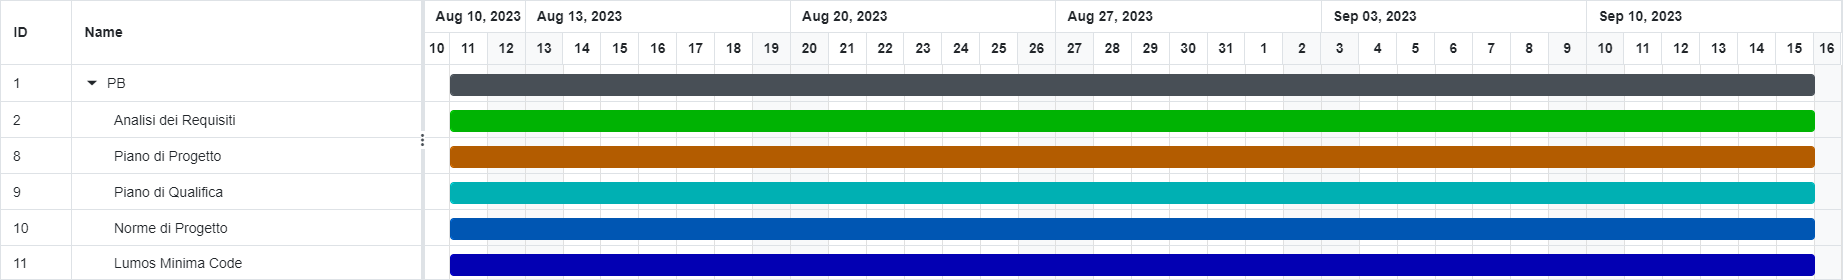
\includegraphics[scale=0.178]{PB_4.png}\newline
\newline
\begin{center}
	\begin{tabularx}{\textwidth}{|X|X|X|X|}
		\hline
		\multicolumn{4}{|c|}{\textbf{Preventivo ore/costi}}                                      \\
		\hline
		\hline
		\textbf{Ruolo}  & \textbf{Costo orario (\euro)} & \textbf{Ore} & \textbf{Prezzo (\euro)} \\
		\hline
		Responsabile    & 30                            & 71(+10)       & 300                      \\
		\hline
		Amministratore  & 20                            & 48(+3)       & 60                      \\
		\hline
		Analista        & 25                            & 100       	& 0                     \\
		\hline
		Progettista     & 25                            & 131       & 0                     \\
		\hline
		Programmatore   & 15                            & 127(+21)      & 315                    \\
		\hline
		Verificatore    & 15                            & 90(+10)       & 150                      \\
		\hline
		\hline
		\textbf{Totale} &                               & 567          & 12120                    \\
		\hline
	\end{tabularx}\\[8pt]
	\mbox{}\\
\end{center}

\begin{center}
	\begin{tabularx}{\textwidth}{|X|X|X|X|X|X|X|}
		\hline
		\multicolumn{7}{|c|}{\textbf{Preventivo ore per membro}}                                            \\
		\hline
		\hline
		\textbf{Membro}   & \textbf{Resp.}    & \textbf{Amm.}   & \textbf{Ana.} &
		\textbf{Proget.}  & \textbf{Program.} & \textbf{Verif.}                                             \\
		\hline
		Alberti Nicolas   & 9(+3)                 & 7(+3)               & 15            & 23  		 & 22(+4) 		 	& 14(+2)      \\
		\hline
		Brotto Romina     & 11(+3)                & 10              	& 17       		& 23    	 & 21(+6)       	& 15(+1) 	\\
		\hline
		Cavaliere Erica   & 10(+2)                & 12             		& 17        	& 21 		 & 22(+3)	 	 	& 15(+1)     \\
		\hline
		Ceccato Francesco & 10(+2)             	  & 5            		& 17            & 22 		 & 22(+4) 			& 16(+2)     \\
		\hline
		Salami Lorenzo    & 10	                & 6              		& 16     		& 23 		 & 21(+2)    	 	& 14(+2)	\\
		\hline
		Soldà Matteo      & 14                    & 6          			& 15            & 22    	 & 22(+2) 			& 14(+2)  	\\
		\hline
		\hline
		\textbf{Totale}   & 73(+10)            & 48(+3)          & 100(+0)        & 131(+0)		 & 131(+21) & 90(+10) \\
		\hline
	\end{tabularx}\\[8pt]
	\mbox{}\\
\end{center}

\newpage

\section{Preventivo delle ore e dei costi}

\subsection{Suddivisione delle ore previste}

\begin{tabular}{|c|c|c|c|c|c|c|c|}
	\hline
	\textbf{}       & \textbf{Respon.} & \textbf{Amministr.} & \textbf{Analista} & \textbf{Proget.} & \textbf{Program.} & \textbf{Verif.} & \textbf{Totale} \\
	\hline
	Erica           & 11               & 9                   & 17                & 21               & 22                & 15              & 95              \\
	\hline
	Francesco       & 12               & 8                   & 16                & 22               & 22                & 15              & 95              \\
	\hline
	Lorenzo         & 12               & 8                   & 16                & 22               & 22                & 15              & 95              \\
	\hline
	Matteo          & 12               & 8                   & 17                & 22               & 21                & 15              & 95              \\
	\hline
	Nicolas         & 11               & 9                   & 17                & 22               & 21                & 15              & 95              \\
	\hline
	Romina          & 12               & 8                   & 17                & 21               & 22                & 15              & 95              \\
	\hline
	\textbf{Totale} & 70               & 50                  & 100               & 130              & 130               & 90              & 570             \\
	\hline
\end{tabular}\\[8pt]

\subsection{Costi attesi}

\begin{tabular}{|c|c|c|c|}
	\hline
	\textbf{Ruolo}                                   & \textbf{Costo orario (\euro)} & \textbf{Ore}                       & \textbf{Prezzo (\euro)} \\
	\hline
	Responsabile                                     & 30                            & 70                                 & 2100                    \\
	\hline
	Amministratore                                   & 20                            & 50                                 & 1000                    \\
	\hline
	Analista                                         & 25                            & 100                                & 2500                    \\
	\hline
	Progettista                                      & 25                            & 130                                & 3250                    \\
	\hline
	Programmatore                                    & 15                            & 130                                & 1950                    \\
	\hline
	Verificatore                                     & 15                            & 90                                 & 1350                    \\
	\hline\hline
	\multicolumn{2}{|c|}{\textbf{Scadenza consegna}} & \textbf{Ore tot.}             & \textbf{Preventivo finale (\euro)}                           \\
	\hline
	\multicolumn{2}{|c|}{15/09/2023}                 & 570                           & 12150                                                        \\
	\hline
\end{tabular}\\[8pt]

\subsection{Grafico dei costi attesi}
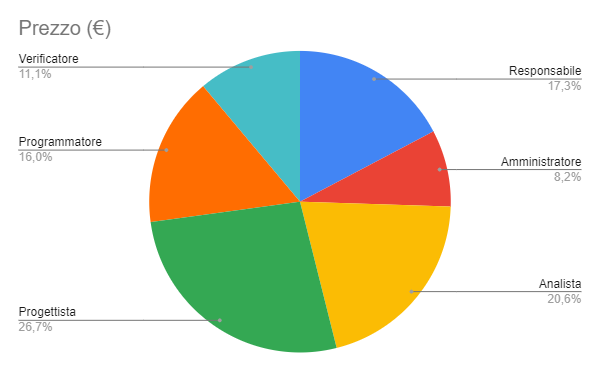
\includegraphics{grafico_costi.png}

\end{document}
